\documentclass[10pt]{article}
\usepackage[utf8]{inputenc}
\usepackage[T1]{fontenc}

\usepackage{amsmath,amssymb,amsfonts,amsthm}
\usepackage[margin=1in, left=1.25in, right=1.25in, top=1in, bottom=1in]{geometry}
\usepackage{booktabs}

\newtheorem{definition}{Definition}
\newtheorem{proposition}{Proposition}
\newtheorem{remark}{Remark}

\usepackage{graphicx}
\usepackage{algorithm}
\usepackage{algorithmic}
\usepackage[linktoc=all, bookmarksdepth=3, pdfstartview=FitH]{hyperref}
\hypersetup{colorlinks=true, linkcolor=blue, filecolor=magenta, urlcolor=cyan}
\urlstyle{same}
\usepackage{multirow}
\usepackage[table,dvipsnames]{xcolor}
\usepackage{subcaption}
\usepackage{caption}
\captionsetup[figure]{name=Figure, labelsep=space}
\captionsetup[table]{labelsep=space}
\usepackage{enumitem}
\usepackage[numbers]{natbib}
\usepackage{cleveref}

\usepackage{placeins}
\makeatletter
\setlength{\@fptop}{0pt}
\setlength{\@fpsep}{14pt}
\setlength{\@fpbot}{0pt plus 1fil}
\renewcommand\paragraph{\@startsection{paragraph}{4}{\z@}%
  {1.0ex plus .2ex minus .1ex}{0.4ex}%
  {\normalfont\normalsize}}
\makeatother
\renewcommand{\algorithmicrequire}{\textup{Require:}}
\renewcommand{\algorithmicensure}{\textup{Ensure:}}
\renewcommand{\algorithmicif}{\textup{if}}
\renewcommand{\algorithmicthen}{\textup{then}}
\renewcommand{\algorithmicelse}{\textup{else}}
\renewcommand{\algorithmicelsif}{\textup{else if}}
\renewcommand{\algorithmicendif}{\textup{end if}}
\renewcommand{\algorithmicfor}{\textup{for}}
\renewcommand{\algorithmicforall}{\textup{for all}}
\renewcommand{\algorithmicdo}{\textup{do}}
\renewcommand{\algorithmicendfor}{\textup{end for}}
\renewcommand{\algorithmicwhile}{\textup{while}}
\renewcommand{\algorithmicendwhile}{\textup{end while}}

% Math commands
% math_commands.tex — shared notation for TransitDuet paper
\newcommand{\R}{\mathbb{R}}
\newcommand{\E}{\mathbb{E}}
\newcommand{\N}{\mathbb{N}}
\DeclareMathOperator*{\argmin}{arg\,min}
\DeclareMathOperator*{\argmax}{arg\,max}

% Policies
\newcommand{\piU}{\pi_{\mathrm{U}}}   % upper policy
\newcommand{\piL}{\pi_{\mathrm{L}}}   % lower policy

% State/action spaces
\newcommand{\sU}{s_{\mathrm{U}}}      % upper state
\newcommand{\sL}{s_{\mathrm{L}}}      % lower state
\newcommand{\aU}{a_{\mathrm{U}}}      % upper action
\newcommand{\aL}{a_{\mathrm{L}}}      % lower action

% Advantages
\newcommand{\AU}{A_{\mathrm{U}}}      % upper advantage
\newcommand{\AL}{A_{\mathrm{L}}}      % lower advantage
\newcommand{\AUaug}{\tilde{A}_{\mathrm{U}}}  % augmented upper advantage
\newcommand{\ALaug}{\tilde{A}_{\mathrm{L}}}  % augmented lower advantage

% Target headway
\newcommand{\htarget}{h^{\mathrm{target}}}
\newcommand{\Hpeak}{H_{\mathrm{peak}}}
\newcommand{\Hoff}{H_{\mathrm{off}}}
\newcommand{\Htrans}{H_{\mathrm{trans}}}

% Measurement / constraint
\newcommand{\zvec}{\mathbf{z}}        % measurement vector
\newcommand{\thetavec}{\boldsymbol{\theta}} % OGD weight vector
\newcommand{\Nfleet}{N_{\mathrm{fleet}}}

% Replay buffer, cost
\newcommand{\D}{\mathcal{D}}          % replay buffer
\newcommand{\climit}{c_{\mathrm{lim}}}
\newcommand{\chigh}{c_{\mathrm{high}}}

% Beta schedule
\newcommand{\betamax}{\beta_{\max}}


\title{TransitDuet: bi-level reinforcement learning for dynamic bus timetable optimisation and holding control}

% \author{Anonymous Authors}
\author{}
\date{}

\begin{document}
\maketitle

\begin{abstract}
Bus timetable planning and real-time holding control are operationally coupled yet typically addressed in isolation. This paper presents TransitDuet, a bi-level reinforcement learning framework that jointly optimises rolling dispatch timetables and station-level holding decisions under stochastic demand and traffic conditions. The upper policy selects discrete planned-headway adjustments that define a dynamic rolling timetable, while the lower policy, a robust ensemble soft actor--critic controller with Lagrangian headway constraints, executes this timetable through station holding. Cross-level coordination operates through a dynamic timetable channel, holding-feedback state augmentation, and per-dispatch hindsight credit assignment, with fleet-size feasibility maintained by measurement-driven online gradient descent penalty adaptation. Evaluated in a calibrated bidirectional bus-corridor microsimulation with elastic fleet budgets across ten random seeds, TransitDuet achieves a mean composite cost of 1.634, which is 3.2\% lower than a target-headway-only variant (1.687) and 11.5\% lower than the best fixed-timetable baseline (1.846). Mean total passenger time is 18.15 minutes, compared with 19.30 and 19.92 minutes for these respective comparators. These results demonstrate that jointly optimising dispatch planning and holding control yields measurable performance gains over single-level holding controllers and decoupled configurations on the evaluated corridor.
\end{abstract}


{\small
\noindent\textbf{Keywords:} bus timetable optimisation; bus holding control; hierarchical reinforcement learning; reinforcement learning; constrained reinforcement learning
}

% Highlights submitted as a separate file (research_highlights.tex).

\section{Introduction}
\label{sec:intro}

High-frequency bus systems face a persistent coordination challenge.
Timetables are planned offline to balance fleet utilisation against passenger demand, yet the headways they prescribe degrade within minutes once buses encounter stochastic traffic and boarding delays.
Real-time holding control can restore regularity, but only within the headway structure it inherits.
When the timetable itself is poorly matched to demand, dispatching too few buses in the peak or too many in the off-peak, holding alone may not recover acceptable service.
Planning and control are thus coupled: the quality of one layer bounds the achievable performance of the other.

Despite this coupling, existing work treats the two problems separately.
The timetable optimisation literature formulates headway or frequency design as mixed-integer programmes solved offline \citep{gkiotsalitis2021bus}, while the holding control literature trains reinforcement learning (RL) agents that take the timetable as given \citep{wang2020real,zhang2026single}.
Joint optimisation would seem a natural application of hierarchical reinforcement learning (HRL), yet three gaps prevent a straightforward application.

\paragraph{Asynchrony between planning and control.}
HRL frameworks such as the options framework \citep{sutton1999between} and goal-conditioned methods such as HIRO \citep{nachum2018data} assume that the upper level sets subgoals or options that can be evaluated through a lower-level execution segment.
In bus operations, the upper policy acts at dispatch events (once per bus departure), while the lower policy acts at every station arrival across all active buses.
The two levels observe different state spaces: the upper level sees route-level demand forecasts and fleet status, whereas the lower level sees per-bus headway deviations and passenger loads.
They also interact through delayed feedback spanning an entire trip lifecycle.
More importantly, several dispatch goals are active concurrently: one upper decision may set the planned launch time of a future trip while buses dispatched under earlier goals continue to move and hold at stations.
Thus the issue is not only the absence of a shared clock, but also the need to optimise and credit overlapping timetable edits.

\paragraph{Cross-advantage under asynchrony.}
Pan et al.~\citep{pan2024roboduet} recently introduced cross-advantage augmentation for bi-level robot locomotion, where an upper style policy and a lower tracking policy execute synchronously on the same state.
Their augmented advantage $\AUaug = \AU + \beta \AL$ directly sums the two advantages at each time step.
This mechanism is not directly applicable when the two levels operate on different timescales with different state and action spaces: no single time step jointly defines $\AU$ and $\AL$.
Generalising cross-level coupling to this asynchronous, multi-timescale setting requires propagating execution outcomes over the variable-length trip lifecycle induced by each dispatch.
It also requires exposing lower-level holding statistics to the upper policy through state augmentation rather than reward backflow.

\paragraph{Fleet and regularity constraints.}
Bus operations also impose feasibility-style constraints, including a fleet-size budget $\Nfleet$ and bounded headway deviation.
Fixed-coefficient reward shaping may not accommodate these constraints reliably.
Constrained RL methods such as reward constrained policy optimisation (RCPO) \citep{tessler2019reward} address single-level constraint satisfaction but do not account for constraints that span a bi-level structure, where the upper level controls resource allocation and the lower level controls service regularity.

\medskip

We propose TransitDuet, a bi-level reinforcement learning framework designed to address these three gaps.
The upper policy $\piU$ selects a discrete planned-headway adjustment for the next same-direction trip; the simulator converts the resulting planned headway into a planned launch time, so the upper directly modifies the rolling timetable. The lower policy $\piL$ is a soft actor-critic (SAC) with Lagrangian penalties \citep{haarnoja2018soft} that selects holding times at each station arrival, with parameters shared across buses.
Two auxiliary upper-only signals---a holding-feedback state channel and a per-dispatch hindsight credit---provide cross-level credit assignment without injecting upper signals into the lower transitions.
Fleet-size feasibility is maintained through $\thetavec$-weighted online gradient descent on a measurement vector, inspired by the ApproPO framework \citep{miryoosefi2019reinforcement}, while headway uniformity enters the lower-level objective through Lagrangian relaxation.

\paragraph{Contributions.}
The specific contributions of this paper are:
\begin{enumerate}
    \item Dynamic timetable--holding formulation. We cast rolling bus timetable optimisation and holding control as a bi-level Markov decision process with heterogeneous state-action spaces and asynchronous transitions.
    \item Discrete timetable and holding policies. The upper policy chooses from a finite dispatch-headway adjustment grid, and the lower policy chooses from a finite holding-time grid augmented with adjacent planned-dispatch context. This discretisation matches operational command granularity and isolates the value of dynamic timetable decisions against fixed-headway baselines.
    \item Adaptive constraint handling via $\thetavec$-weighted online gradient descent (OGD) and Lagrangian relaxation. At the upper level, measurement-driven OGD adjusts the reward weight on fleet overshoot. At the lower level, a dual variable penalises headway deviation. OGD removes the need to hand-tune an overshoot coefficient but provides no worst-case feasibility guarantee.
    \item Empirical evaluation on a calibrated corridor with ten random seeds, reporting both service-quality metrics (waiting time, headway CV, total passenger time) and timetable-execution diagnostics (planned-headway variability, dispatch lateness).
\end{enumerate}

\paragraph{Results preview.}
We evaluate on a high-frequency bus corridor with 22 stations, 264 daily trips, demand stochasticity $\sigma_{\mathrm{demand}} = 0.15$, and elastic fleet $\Nfleet \in [8, 16]$ sampled per episode. All learned methods use the same simulator and random-seed protocol, with the target-headway-only model reported as an ablation rather than as the main TransitDuet configuration.

\section{Related work}\label{sec:related}

\subsection{Reinforcement learning for bus holding control}
\label{subsec:rl_holding}

Research on real-time bus holding spans analytical control rules and learned policies. Early analytical rules remain important reference points. Daganzo~\citep{daganzo2009headway} derived a headway-based control law for eliminating bunching. Xuan et al.~\citep{xuan2011dynamic} proposed dynamic holding strategies that balance schedule reliability and regular headways through optimal linear-control analysis. We include corresponding classical baselines to test whether learning adds value beyond interpretable holding rules.

RL studies learn holding decisions directly from simulated operations. Alesiani and Gkiotsalitis~\citep{alesiani2018reinforcement} formulated high-frequency bus holding as a value-based RL problem. Wang and Sun~\citep{wang2020real} introduced a multi-agent deep RL controller in which each bus acts as an agent under shared training. Zhang et al.~\citep{zhang2026single} developed a single-agent robust deep RL framework for bidirectional timetabled bus lines, showing that categorical identifiers help a shared policy operate across heterogeneous vehicles, stations, and trips.

Subsequent work addressed asynchronous control and robustness. Wang and Sun~\citep{wang2021asynchronous} developed an asynchronous multi-agent reinforcement learning (MARL) framework with counterfactual credit assignment, while Wang and Sun~\citep{wang2023robust} combined distributional MARL with meta-learning to handle service perturbations. Multi-line and multi-strategy settings include shared-corridor multi-objective MARL \citep{wang2023multiobjective}, cooperative holding with stop-skipping \citep{rodriguez2023cooperative}, hierarchical MARL that combines holding and speed control \citep{yu2024hierarchical}, and graph-aware deep RL for multi-line busy corridors \citep{li2026graphaware}.

Other studies focus on RL design choices. He et al.~\citep{he2022dynamic} used Q-learning with multistage look-ahead for adaptive holding. Xu et al.~\citep{xu2025systematic} compared state, action, and agent configurations for RL-based bunching mitigation. Yu et al.~\citep{yu2025llm} used language-model-assisted reward generation for generic bus holding policies. Zhang and Zheng~\citep{resac2026} proposed robust ensemble soft actor-critic (RE-SAC), an ensemble-critic variant of soft actor-critic for bus fleet control that separates aleatoric and epistemic risk signals. We adopt this critic structure at both levels of TransitDuet.

Many RL-based holding controllers treat the timetable, target headway, or dispatch plan as an exogenous input. They can react to realised bunching but do not use systematic execution evidence---such as repeated lateness, excessive onboard delay, or recurrent over-holding---to revise future dispatch times. TransitDuet addresses this limitation by coupling a holding controller with a higher-level rolling timetable policy that feeds execution outcomes back into dispatch planning.

\subsection{Bus timetable optimisation}
\label{subsec:timetable_opt}

Timetable design has traditionally been approached through mathematical programming and metaheuristic search. Ibarra-Rojas et al.~\citep{ibarra2015planning} formulated a mixed-integer programme that jointly determines departure times and vehicle assignments to minimise a weighted combination of passenger waiting time and operator cost. They solved it by branch-and-bound with valid inequalities. Gkiotsalitis and Cats~\citep{gkiotsalitis2021bus} proposed a bi-level model in which the upper level selects headways to minimise total passenger cost and the lower level solves a vehicle-scheduling problem using adaptive large neighbourhood search. Frequency-setting variants, such as the work of Cats and Gl{\"u}ck~\citep{cats2019frequency}, optimise the number of departures per period rather than individual departure times. They typically rely on assignment models to estimate passenger flows under each candidate frequency vector.

Many timetable formulations rely on static demand forecasts and assumed travel-time conditions. They are optimised offline against expected conditions and then handed off to operations without a feedback loop. Under traffic incidents, demand surges, or driver variability, the timetable may become infeasible, leaving holding controllers to absorb the mismatch. The combinatorial structure can also limit scalability as the number of trips and stops increases. TransitDuet instead uses a closed-loop approach in which the upper policy maps aggregate state features to planned-headway adjustments and receives lower-level execution feedback through the cross-level coupling described in Section~\ref{sec:tap}.

\subsection{Hierarchical and multi-timescale reinforcement learning}
\label{subsec:hierarchical_rl}

Hierarchical reinforcement learning decomposes complex tasks across multiple temporal scales. The options framework of Sutton et al.~\citep{sutton1999between} introduced temporally abstract actions, each consisting of an initiation set, an intra-option policy, and a termination condition. It enables planning over multiple timescales within a single Markov decision process (MDP). Feudal networks \citep{vezhnevets2017feudal} operationalize this idea with a manager that sets subgoals in a learned latent space and a worker that executes primitive actions to reach them. HIRO \citep{nachum2018data} introduced off-policy corrections that relabel high-level goals in hindsight, making hierarchical training practical in continuous-control domains. Lee et al.~\citep{lee2020reinforcement} and Metelli et al.~\citep{metelli2020control} studied multi-timescale settings more broadly, including interactions among agents operating at different decision frequencies.

These methods provide useful abstractions for temporal hierarchy, but many assume synchronous execution or a shared state space across levels. In transit operations, the timetable agent acts at dispatch events, whereas the holding agent acts at every stop visit. The two levels therefore observe different state representations at non-aligned decision epochs. TransitDuet handles this asynchrony with a dynamic timetable channel: the upper selects planned-headway adjustments, and the lower executes the resulting timetable through holding.

\subsection{Constrained reinforcement learning}
\label{subsec:constrained_rl}

Many practical RL deployments must satisfy constraints beyond reward maximisation. Lagrangian relaxation is a widely used approach. Tessler et al.~\citep{tessler2019reward} proposed reward-constrained policy optimisation, which augments the policy gradient with dual variables corresponding to cost constraints and performs primal-dual updates to steer the policy toward feasibility. Stooke et al.~\citep{stooke2020responsive} introduced proportional-integral-derivative (PID)-based Lagrange multiplier updates to reduce oscillation and accelerate convergence. These methods handle soft constraints, for which occasional small violations are tolerable, but do not provide worst-case guarantees.

For settings that demand hard constraint satisfaction, Miryoosefi et al.~\citep{miryoosefi2019reinforcement} introduced ApproPO. It formulates the constrained problem as online convex optimisation over occupancy measures and applies a measurement-based projection oracle to enforce feasibility at every iterate. The $\theta$-OGD variant provides a practical implementation that projects policy parameters onto the feasible set using online gradient descent with approximate projections. In the multi-agent domain, Pan et al.~\citep{pan2024roboduet} proposed RoboDuet for humanoid locomotion. Its upper-body controller and lower-body locomotor exchange cross-advantage terms without centralised control.

TransitDuet combines elements from both lines of work to address the constraint structure of transit operations. Fleet-size feasibility is handled as a soft constraint through the $\theta$-OGD measurement-projection scheme of Miryoosefi et al.~\citep{miryoosefi2019reinforcement}. This scheme adaptively reweights an overshoot penalty in the upper-level reward. Per-episode fluctuations under elastic fleet sampling and demand noise can still produce small, bounded overshoot. Headway uniformity is handled as a soft constraint through a Lagrangian penalty with adaptive multiplier updates in the lower-level holding policy. The dynamic timetable channel in Section~\ref{sec:tap} manages cross-level coordination.

\section{Problem formulation}
\label{sec:problem}

We formulate dynamic timetable optimisation and holding control as a bi-level Markov decision process (MDP) for a single bus route with time-varying passenger demand. The upper level makes rolling dispatch-time decisions by selecting a planned-headway adjustment for the next same-direction trip. The lower level executes the resulting dynamic timetable through real-time holding decisions.
This section defines the problem variables, action spaces, measurements, and interaction structure used in the experiments. The learning architecture and training mechanisms are specified in \Cref{sec:method}.

%% ---------------------------------------------------------------
\subsection{Bus transit system model}
\label{sec:transit_model}

We consider a single bidirectional bus route consisting of $M$ stations indexed $\{1,\dots,M\}$.
Service is provided according to a timetable that dispatches a total of 264~trips per day, alternating between the two directions.
Passenger demand is drawn from time-varying origin--destination (OD) matrices that capture morning, midday, and evening peaks.
At any point in time, at most $\Nfleet^{\max}=25$ buses may be concurrently in service; each trip is characterized by a baseline launch time, a planned launch time, an actual launch time, and a travel direction.
The planned same-direction dispatch headway is the timetable lever, while per-station holding times constitute the real-time control lever.

%% ---------------------------------------------------------------
\subsection{Bi-level MDP formulation}
\label{sec:bilevel_mdp}

We decompose the joint optimisation into two coupled MDPs that share a common environment but differ in observation granularity, action semantics, and decision frequency.

\subsubsection{Upper-level MDP (dynamic timetable planning)}
\label{sec:upper_mdp}

The upper-level policy $\piU$ selects a planned-headway adjustment for the next same-direction dispatch.
It is invoked after each successful dispatch event ($M \approx 264$ events per episode, $\approx 132$ per direction; one episode is one full service day), so its sampling cadence is event-driven rather than a fixed wall-clock timer.

\paragraph{State.}
The upper state encodes system-level summary statistics and the holding-feedback (HoldFB) block that closes the lower-to-upper loop (\Cref{sec:tap}):
{\small
\begin{equation}
  \label{eq:upper_state}
  \begin{aligned}
    \sU = \bigl[\,
      &\underbrace{\tfrac{\text{hour}}{24},\,
                   \tfrac{\text{demand}}{1000},\,
                   \tfrac{\text{fleet\_on\_route}}{\Nfleet^{\max}},\,
                   \tfrac{\text{prev\_headway}}{600},\,
                   \text{holding\_ratio}}_{\text{system summary, dims 0--4}},\\[-1pt]
      &\underbrace{\tfrac{\bar{h}^{\mathrm{up}}_{\mathrm{hold}}}{60},\,
                   \tfrac{\sigma^{\mathrm{up}}_{\mathrm{hold}}}{60},\,
                   \tfrac{\bar{h}^{\mathrm{down}}_{\mathrm{hold}}}{60}}_{\text{HoldFB, dims 5--7}},\,
       \underbrace{\tfrac{\htarget}{600},\,\mathrm{dir},\,\tfrac{\Nfleet}{20}}_{\text{trip context, dims 8--10}}
    \,\bigr] \;\in\; \R^{11}.
  \end{aligned}
\end{equation}
}
where each component is normalised to facilitate learning. Dims 5--7 are the rolling holding statistics over the last 10 completed trips (see~\Cref{sec:tap}); the $-$HoldFB ablation in~\Cref{sec:ablation} zeroes these three dimensions. Dim 10 is the per-episode elastic fleet budget $\Nfleet \in [8, 16]$, which the policy must condition on when choosing planned headways under different fleet budgets.

\paragraph{Action.}
After trip $k-1$ in a direction is dispatched at actual time $\tau^{\mathrm{act}}_{k-1}$, the upper policy selects a scalar planned-headway adjustment:
\begin{equation}
  \label{eq:upper_action}
  \aU = \Delta h_k \in \{-60,-30,0,30,60\}\;\text{s}.
\end{equation}
The planned headway and planned launch time are
\begin{equation}
  \label{eq:timetable_action}
  h^{\mathrm{plan}}_k =
  \mathrm{clip}(300 + \Delta h_k, 240, 360),\qquad
  \tau^{\mathrm{plan}}_k =
  \max(\tau^{\mathrm{act}}_{k-1}+h^{\mathrm{plan}}_k,\; t+60).
\end{equation}
The baseline timetable is retained only as a reference for reporting planned shifts $\tau^{\mathrm{plan}}_k-\tau^{\mathrm{base}}_k$; it no longer constrains dispatch once the dynamic timetable policy is active.
If fleet availability or the soft fleet ceiling delays a planned dispatch, the realised lateness is recorded as $\tau^{\mathrm{act}}_k-\tau^{\mathrm{plan}}_k$.
The lower controller then receives $h^{\mathrm{plan}}_k$ as the trip-specific headway target.

\paragraph{Reward.}
The upper reward is computed at the episode level from a measurement vector (defined in \Cref{sec:constraints}).
Because each upper action influences the system over an extended horizon through the downstream holding decisions it induces, assigning credit to individual dispatch events is nontrivial; we defer the reward construction to~\Cref{sec:method}.

\subsubsection{Lower-level MDP (holding control)}
\label{sec:lower_mdp}

The lower-level policy $\piL$ decides how long each bus should dwell beyond its minimum stop time at every station.
A decision is triggered at each station arrival for each active bus, producing a high volume of decision epochs throughout the day.

\paragraph{State.}
The lower state captures the local context of an individual bus:
\begin{equation}
  \label{eq:lower_state}
  \begin{aligned}
    \sL = \bigl[\,
      &\text{bus\_id},\,
       \text{station\_id},\,
       \text{hour},\,
       \text{direction},\\
      &h_{\mathrm{fwd}},\,
       h_{\mathrm{bwd}},\,
       \hat{d},\,
       \Delta h,\,
       a_{\mathrm{last}},\,
       h^{\mathrm{plan}}_k,\,
       h^{\mathrm{plan}}_{k-1},\,
       h^{\mathrm{plan}}_{k+1},\,
       \rho_{\mathrm{station}},\,
       v_1,\dots,v_K
    \,\bigr] \;\in\; \R^{13+K},
  \end{aligned}
\end{equation}
where $h_{\mathrm{fwd}}$ and $h_{\mathrm{bwd}}$ denote the forward and backward headways, $\hat{d}$ is the estimated dwell time, $\Delta h$ is the deviation of the current headway from the planned trip headway, $a_{\mathrm{last}}$ is the previous holding action, $h^{\mathrm{plan}}_{k-1:k+1}$ encode adjacent planned dispatch gaps, $\rho_{\mathrm{station}}$ is station progress, and $v_1,\dots,v_K$ are recent inter-station speeds that encode local traffic conditions.

\paragraph{Action.}
The lower action is a scalar holding time selected from the operational grid used by the final policy:
\begin{equation}
  \label{eq:lower_action}
  \aL \;\in\; \{0,3,6,9,12,15,20,30\}\;\text{seconds}.
\end{equation}

\paragraph{Reward and cost.}
The immediate lower reward is a function of headway deviation from the target set by the upper level.
We define the per-step cost as
\begin{equation}
  \label{eq:lower_cost}
  c(\sL,\aL) = \min\!\Bigl(\frac{(h_{\mathrm{fwd}} - \htarget)^{2}}{(\htarget)^{2}},\;1\Bigr),
\end{equation}
which penalises headway irregularity in a scale-invariant manner and is clipped at~1 for numerical stability.

%% ---------------------------------------------------------------
\subsection{Constraint specification}
\label{sec:constraints}

The bi-level MDP is subject to two soft constraints, both evaluated through a measurement vector collected at the end of each episode.

\paragraph{Measurement vector.}
At the conclusion of a service day, we compute:
\begin{equation}
  \label{eq:measurement}
  \zvec = \bigl[\,\text{avg\_wait\_min},\;\text{peak\_fleet},\;\text{headway\_CV}\,\bigr].
\end{equation}

\paragraph{Soft constraint (fleet budget).}
The peak number of buses simultaneously on route should respect the per-episode fleet budget $\Nfleet \in [\Nfleet^{\min}, \Nfleet^{\max}]$ sampled at episode start. We enforce this softly via an overshoot$^2$ penalty in the upper reward:
\begin{equation}
  \label{eq:soft_fleet}
  \mathrm{overshoot}(\zvec, \Nfleet) = \max(0,\, \text{peak\_fleet} - \Nfleet)^2,
\end{equation}
weighted by an adaptive coefficient maintained by $\thetavec$-OGD (see~\Cref{sec:meas_proj}). To prevent unbounded violation under noisy demand, the environment imposes an outer ceiling $\Nfleet^{\max} + 3$ buses, which bounds but does not zero out the realised overshoot.

\paragraph{Soft constraint (headway uniformity).}
The expected per-step cost must remain below a threshold:
\begin{equation}
  \label{eq:soft_constraint}
  \E_{\piU,\piL}\!\bigl[\,c(\sL,\aL)\,\bigr] \;\leq\; \climit,
\end{equation}
which encourages even spacing of buses along the route.
Satisfaction of this constraint is enforced via Lagrangian relaxation within the lower-level policy (see \Cref{sec:method}).

%% ---------------------------------------------------------------
\subsection{Timescale separation}
\label{sec:timescale}

The principal characteristic of the bi-level formulation is the pronounced separation of timescales between the two decision layers.
The upper policy $\piU$ acts at dispatch events, which occur roughly every five~minutes on average.
The lower policy $\piL$, by contrast, acts at every station arrival for every active bus, a frequency on the order of once every 30~seconds system-wide when multiple buses are in service.
Consequently, hundreds of lower-level decisions may intervene between two consecutive upper-level decisions, and the two layers never act simultaneously.

This asynchrony distinguishes our setting from the semi-Markov options framework~\citep{sutton1999between} and feudal reinforcement learning~\citep{dayan1992feudal,vezhnevets2017feudal}, which assume that (i)~the manager and worker share a common state space or a fixed abstraction thereof, and (ii)~the manager selects a subgoal that the worker executes to completion before the manager acts again.
Neither assumption holds here: the upper state $\sU\in\R^{11}$ summarises fleet-level statistics plus the HoldFB block whereas the lower state $\sL\in\R^{13+K}$ encodes bus-level kinematics, timetable context, and local traffic conditions, and both policies issue decisions driven by environment events rather than by a synchronous clock or a predefined option duration.

More concretely, a single upper action (a planned-headway adjustment $\Delta h_k$) determines the planned launch time for the next dispatch while many buses traverse multiple stations under independent lower-level control. The upper policy cannot pause and wait for all induced lower decisions to conclude.
Standard HRL methods that propagate value or advantage across levels therefore require modification to handle the fully asynchronous, event-driven interaction between $\piU$ and $\piL$.
We address this challenge through a dynamic-timetable coupling, detailed in \Cref{sec:method}.

\paragraph{Relation to goal-conditioned options.}
One can view a dispatched bus as carrying an active goal, namely its planned headway $h^{\mathrm{plan}}_k$, and the lower policy is indeed conditioned on that goal.
However, this interpretation alone does not express the part of the problem that TransitDuet optimises.
The upper action is not an option assigned to a bus and terminated when that bus reaches a goal. It is a rolling timetable adjustment that determines the planned launch time of a future trip, sometimes before the corresponding vehicle is available, while other buses continue executing previously planned trips.
Multiple planned headways are therefore active concurrently, and their effects interact through station-level holding, fleet availability, and dispatch lateness.
A conventional goal-conditioned option model with a shared $\pi(\aL\mid\sL,o_i)$ can represent the lower tracking controller, but it does not by itself specify how future dispatch times are generated, how timetable feasibility is audited, or how credit from passenger wait, onboard delay, and fleet overshoot is assigned back to asynchronous dispatch-time decisions.

\section{TransitDuet framework}
\label{sec:method}

TransitDuet comprises an upper timetable policy and a lower holding policy linked by a dynamic timetable channel. \Cref{fig:arch} summarises the architecture; the following subsections specify policy training, cross-level coupling, adaptive fleet-overshoot penalties, and the target-headway-only ablation.

\begin{figure}[H]
    \centering
    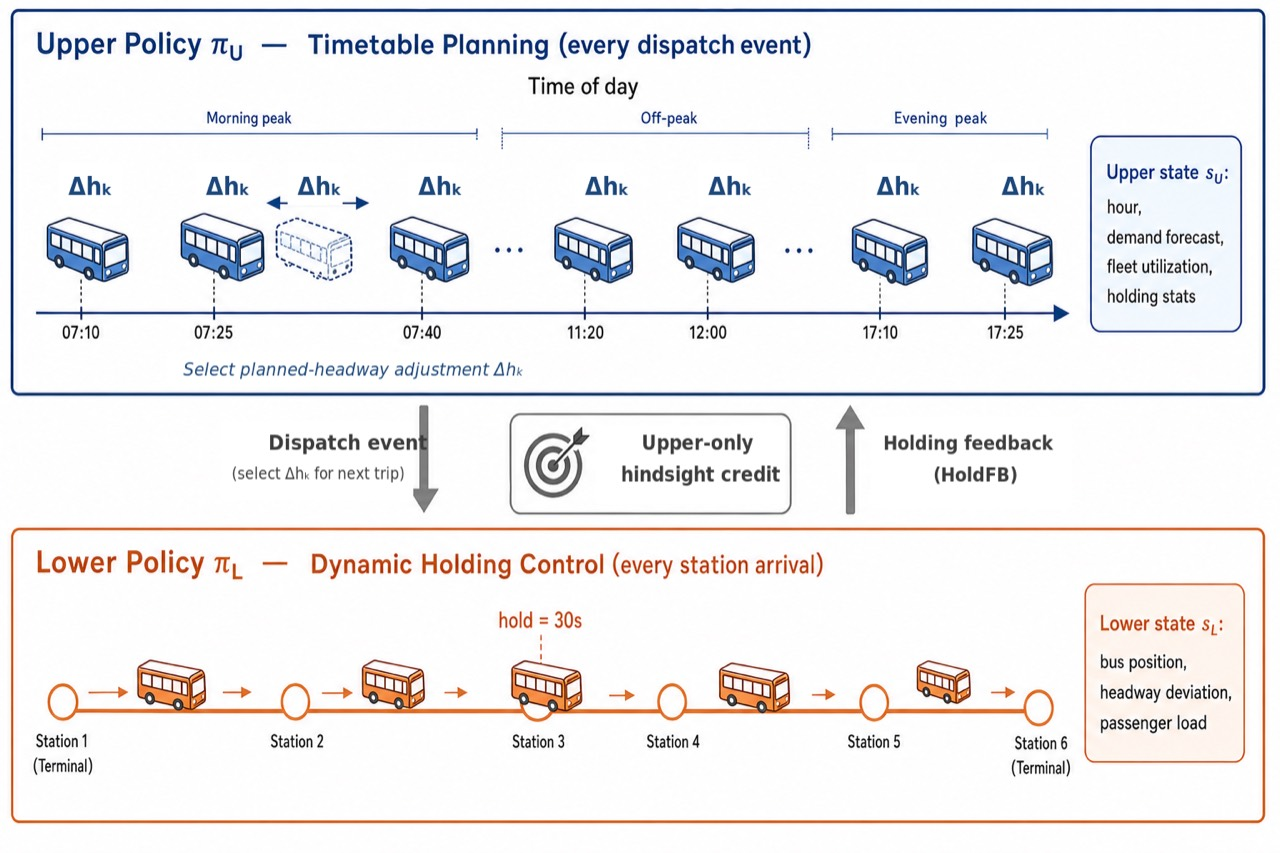
\includegraphics[width=0.92\textwidth]{figures/architecture_user_supplied.jpg}
    \caption{TransitDuet bi-level architecture. The upper policy $\piU$ selects a planned-headway adjustment after each dispatch event; the lower policy $\piL$ selects a holding duration at each station arrival.}
    \label{fig:arch}
\end{figure}

%% ====================================================================
\subsection{Architecture overview}
\label{sec:arch}

TransitDuet comprises two independent policy networks operating at different timescales and over different state-action spaces.
The upper policy $\piU$ is a lightweight categorical multilayer perceptron (MLP) that selects a planned-headway adjustment for the next same-direction dispatch.
The lower policy $\piL$ is a discrete RE-SAC--Lagrangian controller that selects holding durations at every station arrival, with parameters shared across all buses.

A key design choice is that the two networks share no encoder parameters.
This differs from the shared-body, dual-head architecture of RoboDuet \citep{pan2024roboduet}, which couples an upper style policy and a lower tracking policy through a common proprioceptive encoder.
Shared encoders are appropriate when the two levels observe the same state at each time step, as in synchronous robot locomotion, but are ill-suited here for two reasons.
First, $\sU$ and $\sL$ live in different spaces: $\sU$ encodes route-level demand forecasts and fleet status, whereas $\sL$ encodes per-bus headway deviation, passenger load, and local occupancy.
Second, the two levels are triggered asynchronously.
The upper policy acts once per dispatch event (roughly once per $\htarget$ seconds), while the lower policy acts at every station arrival of every active bus, producing hundreds of decisions per upper-level step.
Forcing these heterogeneous signals through a shared trunk would create conflicting gradient directions.

The two levels communicate through a dynamic timetable channel (\cref{sec:tap}).
Both networks are trained with off-policy soft actor-critic. The RE-SAC upper reuses per-dispatch transitions from a replay buffer, while the lower uses the same ensemble structure with a Lagrangian dual variable for headway-constraint satisfaction.

%% ====================================================================
\subsection{Upper-level timetable policy}
\label{sec:upper}

The upper policy $\piU$ maps the route-level state $\sU$ to a discrete planned-headway adjustment $\Delta h \in \{-60,-30,0,30,60\}$\,s.
After a trip is dispatched, this adjustment defines the planned headway and planned launch time of the next same-direction trip according to \Cref{eq:timetable_action}.
The lower's Lagrangian cost (Section~\ref{sec:lower}) is then computed against this dispatch-specific planned headway.

\paragraph{Network architecture.}
The policy is parameterised as a two-layer MLP with 64 hidden units per layer and rectified linear unit (ReLU) activations, followed by categorical logits over the five timetable actions:
\begin{equation}
\label{eq:upper_net}
    \ell_{\phi}(\sU) = W_3 \, \mathrm{ReLU}(W_2 \, \mathrm{ReLU}(W_1 \sU + b_1) + b_2) + b_3 .
\end{equation}
The action distribution is
\begin{equation}
\label{eq:upper_action_method}
    \piU(\Delta h \mid \sU) =
    \mathrm{Categorical}\!\left(\mathrm{softmax}(\ell_{\phi}(\sU))\right).
\end{equation}

\paragraph{Off-policy SAC training (RE-SAC upper).}
The upper policy is trained as an off-policy soft actor-critic with an ensemble of $K{=}10$ Q-networks and a lower-confidence-bound (LCB) value in the policy-improvement step. This is the same RE-SAC-style structure~\citep{resac2026} used at the lower level (\cref{sec:lower}), without the Lagrangian. Each dispatch event $i$ contributes a transition $(s_{\mathrm{U},i}, a_{\mathrm{U},i}, R_{\mathrm{U}}^{(i)}, s_{\mathrm{U},i+1}, d_i)$ to a 50k-capacity replay buffer. The per-dispatch reward $R_{\mathrm{U}}^{(i)}$ is the hindsight-credited reward of \Cref{eq:hindsight_reward} (\cref{sec:tap}). The ensemble Q-networks are trained against a single shared mean target to prevent ensemble divergence,
{\footnotesize
\begin{equation}
\label{eq:upper_q_target}
    y_i = R_{\mathrm{U}}^{(i)} + \gamma(1-d_i)\!\left(\frac{1}{K}\sum_{k=1}^{K}\bar{Q}_{k}(s_{\mathrm{U},i+1},\tilde{a}) - \alpha_{\mathrm{U}}\log\piU(\tilde{a}\mid s_{\mathrm{U},i+1})\right).
\end{equation}
}
where $\bar{Q}_{k}$ is the $k$-th target network and $\tilde{a} \sim \piU(\cdot\mid s_{\mathrm{U},i+1})$. The target is clamped to $[-50, 50]$. For the categorical policy, the target value is the probability-weighted expectation over the five action bins. The per-Q mean-squared-error (MSE) loss is augmented with a small ensemble-spread penalty $\beta_{\mathrm{ood}} \cdot \mathrm{std}_k(Q_k)$ that encourages the ensemble to disagree on out-of-distribution actions. The policy is improved by maximizing the LCB value:
{\footnotesize
\begin{equation}
\label{eq:upper_policy_loss}
    \mathcal{L}_{\piU}(\phi) = \mathbb{E}_{s\sim\mathcal{D}_{\mathrm{U}},\,a\sim\piU}\!\left[\alpha_{\mathrm{U}}\log\piU(a\mid s) - \bigl(\bar{Q}(s,a) + \beta_{\mathrm{LCB}}\sigma_Q(s,a)\bigr)\right].
\end{equation}
}
where $\beta_{\mathrm{LCB}} = -2$, so the LCB value $\bar{Q} + \beta_{\mathrm{LCB}}\sigma_Q$ subtracts twice the ensemble disagreement from the mean. Auto-entropy adjusts $\alpha_{\mathrm{U}}$ toward the categorical target entropy. We use an off-policy SAC upper because dispatches are scarce ($M\!\approx\!264$ per episode), allowing a replay buffer to reuse each transition across gradient updates.

%% ====================================================================
\subsection{Lower-level holding control policy}
\label{sec:lower}

The lower policy $\piL$ selects a non-negative holding action from the grid $\{0,3,6,9,12,15,20,30\}$ seconds at each station arrival.
It is trained with a discrete soft actor-critic controller augmented by a Lagrangian cost term for headway-deviation constraint enforcement \citep{haarnoja2018soft}.
All buses share the same policy parameters, allowing the controller to operate across the fleet from bus-specific input states.

\paragraph{Categorical holding policy.}
A two-layer MLP with 64 hidden units per layer and ReLU activations produces categorical logits over the eight holding bins. The discrete formulation avoids asking the actor to learn distinctions smaller than the simulator time resolution and makes the action interface match practical holding commands.

\paragraph{Reward Q-ensemble (RE-SAC, $K{=}10$).}
Rather than the standard twin-Q double-clipped critic of SAC, the lower uses the RE-SAC critic of Zhang and Zheng~\citep{resac2026}. It replaces the double clip with an ensemble of $K{=}10$ independently initialized Q-networks $\{Q_{\omega_k}\}_{k=1}^{K}$, each a two-layer MLP with 64 hidden units. It also uses a lower-confidence bound rather than the minimum of the two critics for policy improvement. To prevent ensemble divergence, all members are trained against a single shared mean target,
{\footnotesize
\begin{equation}
\label{eq:lower_q_target}
    y = r + \gamma\!\left(\frac{1}{K}\sum_{k=1}^{K}Q_{\bar{\omega}_k}(\sL',\aL') - \alpha\log\piL(\aL'\mid\sL')\right).
\end{equation}
}
with $\aL' \sim \piL(\cdot \mid \sL')$,
and the per-$Q_k$ loss is augmented with a small ensemble-spread regulariser,
{\footnotesize
\begin{equation}
\label{eq:lower_q_loss}
    \mathcal{L}_Q(\omega_k) = \E_{(\sL,\aL,r,\sL')\sim\D}\!\left[\bigl(Q_{\omega_k}(\sL,\aL)-y\bigr)^2\right] + \beta_{\mathrm{ood}}\,\mathrm{std}_k\bigl(Q_{\omega_k}(\sL,\aL)\bigr).
\end{equation}
}
with $\beta_{\mathrm{ood}} = 0.1$,
which encourages members to disagree on out-of-distribution actions. Target parameters $\bar{\omega}_k$ track $\omega_k$ via Polyak averaging with $\tau = 0.005$. Policy improvement is performed against the ensemble lower-confidence bound (LCB),
\begin{equation}
\label{eq:lower_lcb}
    \bar{Q}(s, a) = \tfrac{1}{K}\sum_{k} Q_{\omega_k}(s, a),\qquad \sigma_Q(s, a) = \mathrm{std}_k\bigl(Q_{\omega_k}(s, a)\bigr).
\end{equation}
A standard SAC twin-Q critic corresponds to the special case $K{=}2$ without the LCB; we use the $K{=}10$ ensemble to represent uncertainty in the lower actor loss below.

\paragraph{Cost Q-network and Lagrangian relaxation.}
A separate single-MLP cost critic $Q^c_{\xi}(\sL, \aL)$ (same hidden width 64) estimates the expected cumulative headway-deviation cost. The lower-level actor loss balances entropy, the ensemble LCB value, and the constraint:
{\footnotesize
\begin{equation}
\label{eq:lower_policy_loss}
    \mathcal{L}_{\piL}(\psi) = \E_{\sL\sim\D,\,\aL\sim\piL}\!\left[\alpha\log\piL(\aL\mid\sL) - \bigl(\bar{Q}(\sL,\aL)+\beta_{\mathrm{LCB}}\sigma_Q(\sL,\aL)\bigr) + \lambda Q^c_{\xi}(\sL,\aL)\right].
\end{equation}
}
with $\beta_{\mathrm{LCB}} = -2$ (the policy is improved against the lower confidence bound) and $\lambda \geq 0$ the Lagrange multiplier. The dual is updated to satisfy the cost-limit constraint $\climit$:
\begin{equation}
\label{eq:lambda_update}
    \lambda \leftarrow \exp\!\left[\mathrm{clamp}\!\left(\log\lambda + \eta_{\lambda}\bigl(\E[Q^c_{\xi}]-\climit\bigr),\,-10,\,5\right)\right].
\end{equation}
with $\eta_{\lambda} = 10^{-4}$.
Updating in log-space ensures $\lambda > 0$ and the clamp prevents numerical instability.

\paragraph{Auto-entropy tuning.}
The temperature $\alpha$ is adjusted to maintain a target entropy $\bar{\mathcal{H}} = -\dim(\aL) = -1$:
\begin{equation}
\label{eq:alpha_update}
    \alpha \leftarrow \min\!\Bigl(\alpha_{\max}^{\mathrm{L}},\; \exp\!\bigl(\log\alpha - \eta_{\alpha}\,(\log \piL(\aL \mid \sL) + \bar{\mathcal{H}})\bigr)\Bigr),
\end{equation}
with $\alpha_{\max}^{\mathrm{L}} = 0.08$ to prevent entropy collapse while the timetable and holding policies co-adapt.

%% ====================================================================
\subsection{Cross-level coupling: dynamic timetable design}
\label{sec:tap}

TransitDuet couples the two policies through a dynamic timetable channel. The upper selects a planned-headway adjustment, the environment converts it into a planned launch time, and the lower's Lagrangian cost is computed against the planned headway of the dispatched trip. A target-headway-only channel is included as an ablation variant that changes the lower reference headway without altering planned dispatch times.

\paragraph{Timetable channel: planned dispatch headway.}
At each dispatch event, the upper outputs $\Delta h_k$ and sets $h^{\mathrm{plan}}_k$ and $\tau^{\mathrm{plan}}_k$ via \Cref{eq:timetable_action}. The lower's Lagrangian constraint becomes
\begin{equation}
\label{eq:goal_constraint}
    \E_{\tau \sim \pi_{\mathrm{L}}}\!\!\left[\,\big|H_{\mathrm{real}}(\tau) - h^{\mathrm{plan}}_k\big|\right] \;\leq\; \chigh,
\end{equation}
where $H_{\mathrm{real}}(\tau)$ is the realised inter-bus headway over the trip lifecycle $\tau$. The upper policy thereby defines an executable rolling timetable rather than only a soft tracking target.

\paragraph{State channel: holding feedback (HoldFB).}
The upper state $\sU$ contains a 3-dimensional holding-feedback block at indices 5--7 (Eq.~\ref{eq:upper_state}; Section~\ref{sec:aux}). It carries a rolling 10-trip summary of the lower policy's recent holding decisions: $[\bar{h}^{\mathrm{up}}_{\mathrm{hold}}, \sigma^{\mathrm{up}}_{\mathrm{hold}}, \bar{h}^{\mathrm{down}}_{\mathrm{hold}}]$, normalised to the action range. This channel exposes the intensity of lower-level intervention to the upper policy, allowing it to adapt $\Delta h_k$ in response to sustained holding.

\paragraph{Reward channel: trip-lifecycle hindsight credit.}
At episode end, we compute the realised inter-dispatch gap $g_i$ for each dispatch $i$ from the actual launch times of each bus. We then form a per-dispatch deviation $\Delta_i = |g_i - \bar{g}|/\sigma_g$, where $(\bar{g}, \sigma_g)$ are the per-direction mean and standard deviation. The upper reward at dispatch $i$ combines the episode-level system reward with a per-dispatch hindsight credit:
\begin{equation}
\label{eq:hindsight_reward}
    R_{\mathrm{U}}^{(i)} = R_{\mathrm{sys}}(\zvec) - \alpha_{\mathrm{H}} \cdot \frac{\Delta_i - \bar{\Delta}}{\sigma_{\Delta}}, \qquad \alpha_{\mathrm{H}} = 0.5,
\end{equation}
where $R_{\mathrm{sys}}$ is the belief-weighted multi-objective reward (Eq.~\ref{eq:morl_reward}). The second term recentres the deviation across the episode, so dispatches whose realised lifecycles produced more regular gaps than the episode average earn positive credit. This is upper-only credit assignment; no signal flows back into the lower transitions.

\paragraph{Lower-level reward.}
The lower reward is unchanged from Section~\ref{sec:lower}: it is the standard environment reward augmented by the Lagrangian headway-deviation cost. Upper coupling redirects the constraint target in Eq.~\ref{eq:goal_constraint} to the current trip's planned headway. We do not inject upper-level reward signals into lower transitions. Advantage-based auxiliary-reward and target-headway-only channels are retained as comparison rows \citep{li2019hierarchical,singh2024piper}.

\paragraph{Training-stage schedule.}
Cross-level coupling is gated by a two-stage schedule. During the first $e_{\mathrm{warm}} = 15$ episodes, the upper policy is inactive and the lower trains against a fixed 300-second rolling timetable. From episode $e_{\mathrm{warm}}$ onward, the upper activates and selects planned-headway adjustments. The state and reward channels operate only on the upper side and are inactive during warmup by construction.

%% ====================================================================
\subsection{Adaptive fleet-overshoot penalty}
\label{sec:meas_proj}

The upper policy must respect operational targets on fleet size, average passenger waiting time, and headway regularity.
Rather than adding fixed penalty terms to the reward, we use an adaptive scheme inspired by the ApproPO framework \citep{miryoosefi2019reinforcement}. A measurement-driven online gradient descent ($\thetavec$-OGD) update of the reward-weight vector adjusts relative penalty strengths from realised episode statistics. Unlike full ApproPO, our scheme does not solve a nested best-response oracle and does not provide ApproPO's feasibility guarantees. It reweights the reward toward the measurements furthest from their targets. In the reported experiments, fleet overshoot remains bounded but is not driven to zero (\cref{sec:experiments}).

\paragraph{Measurement vector.}
At the end of each episode, we compute a three-dimensional measurement vector:
\begin{equation}
\label{eq:measurement_method}
    \zvec = \bigl[\bar{w},\; n_{\mathrm{peak}},\; \mathrm{CV}_{h}\bigr] \in \R^3,
\end{equation}
where $\bar{w}$ is the average passenger waiting time, $n_{\mathrm{peak}}$ is the peak fleet size (maximum number of buses simultaneously in service), and $\mathrm{CV}_{h}$ is the coefficient of variation of realised headways.

\paragraph{Weight vector and reward modulation.}
A weight vector $\thetavec \in \R^3$, initialized as $\thetavec_0 = [-0.5,\, -0.3,\, -0.2]$, modulates the upper-level reward:
\begin{equation}
\label{eq:upper_reward}
\begin{aligned}
    R_{\mathrm{U}} &= \thetavec^\top \mathbf{p},\\
    \mathbf{p} &= \bigl[\bar{w},\; (\max(0,\, n_{\mathrm{peak}} - \Nfleet))^2,\; \mathrm{CV}_{h}\bigr].
\end{aligned}
\end{equation}
The quadratic penalty on fleet overshoot $(\max(0,\, n_{\mathrm{peak}} - \Nfleet))^2$ ensures that small violations incur proportionally less cost than large ones, providing a smooth gradient.

\paragraph{Online gradient descent update.}
The weight vector is updated by online gradient descent (OGD) on a loss that drives each measurement toward its target:
\begin{equation}
\label{eq:ogd_loss}
    \ell_t = \bigl[-\bar{w}_t,\; -\max(0,\, n_{\mathrm{peak},t} - \Nfleet),\; -\mathrm{CV}_{h,t}\bigr],
\end{equation}
\begin{equation}
\label{eq:ogd_update}
    \thetavec_{t+1} = \Pi_{\mathcal{B}}\!\bigl(\thetavec_t + \eta_t \, \ell_t\bigr), \quad \eta_t = \frac{\eta_0}{\sqrt{t}},
\end{equation}
where $\Pi_{\mathcal{B}}$ projects onto the unit ball $\{\thetavec : \|\thetavec\|_2 \leq 1\}$ and $\eta_0$ is the base learning rate.
The $1/\sqrt{t}$ schedule follows standard online convex optimisation analysis, in which projected OGD on a convex loss has an $O(\sqrt{T})$ regret bound and sublinear cumulative constraint violation. We do not claim the same guarantee for the learned policy. The inner optimisation is a non-convex SAC update on a replay buffer rather than the convex best-response oracle required by ApproPO, and we do not project onto an occupancy-measure feasibility set. We therefore use $\thetavec$-OGD as an adaptive penalty whose feasibility properties for the resulting deep-RL policy are empirical rather than provable.

The simplification relative to ApproPO is deliberate. Because the upper policy is trained off-policy with the $\thetavec$-modulated reward, repeated SAC gradient updates on the replay buffer act as an approximate best-response step. This eliminates the inner optimisation loop that ApproPO requires, at the cost of the formal guarantee discussed above.

%% ====================================================================
\subsection{Training procedure}
\label{sec:training}

\Cref{alg:training} presents the full TransitDuet training loop, which coordinates the upper-warmup schedule with the upper and lower policy updates, the cross-level coupling channels of \cref{sec:tap}, and the measurement projection.

\begin{algorithm}[t]
\caption{TransitDuet training procedure}
\label{alg:training}
\begin{algorithmic}[1]
\REQUIRE Episode budget $E$, upper warmup $e_{\mathrm{warm}} = 15$, lower update frequency $f_{\mathrm{L}}$, batch size $B$, hindsight credit weight $\alpha_{\mathrm{H}}$
    \STATE Initialize upper policy $\piU$, lower policy $\piL$ (RE-SAC ensemble of $K{=}10$ reward critics + single cost critic), replay buffer $\D$, Lagrange multiplier $\lambda$, entropy temperature $\alpha$, $\thetavec$-OGD weights, exponential-moving-average (EMA) target upper $\bar{\piU}$
\FOR{episode $e = 1, \ldots, E$}
    \STATE Reset simulation; sample $\Nfleet \sim \mathrm{Uniform}\{8, \ldots, 16\}$ if elastic
    \STATE $\mathcal{T}_{\mathrm{U}} \leftarrow \emptyset$, $\mathcal{T}_{\mathrm{L}} \leftarrow \emptyset$
    \WHILE{episode not done}
        \IF{dispatch event triggered}
            \IF{$e \leq e_{\mathrm{warm}}$}
                \STATE Use fixed $300$\,s planned headway (upper inactive)
            \ELSE
                \STATE Sample $\Delta h_k \sim \piU(\cdot\mid\sU)$; set $h^{\mathrm{plan}}_k$ and $\tau^{\mathrm{plan}}_k$ via \cref{eq:timetable_action}
                \STATE Record $(s_{\mathrm{U},i}, a_{\mathrm{U},i})$ in $\mathcal{T}_{\mathrm{U}}$
            \ENDIF
        \ENDIF
        \IF{station arrival for any bus $b$}
            \STATE Observe $\sL$; sample $\aL \sim \piL(\cdot \mid \sL)$; apply holding $\aL$
            \STATE Observe $r_{\mathrm{L}}, c_{\mathrm{L}}, \sL'$; store $(\sL, \aL, r_{\mathrm{L}}, c_{\mathrm{L}}, \sL')$ in $\D$ and $\mathcal{T}_{\mathrm{L}}$
            \IF{step $\bmod\; f_{\mathrm{L}} = 0$ \AND $|\D| \geq B$}
                \STATE Sample $B$ transitions from $\D$
                \STATE Update $\piL$ critics, policy, $\lambda$, $\alpha$ via SAC losses
                \STATE Soft-update lower target networks
            \ENDIF
        \ENDIF
    \ENDWHILE
    \STATE Compute episode measurements $\zvec$, system reward $R_{\mathrm{sys}}$, and per-dispatch hindsight credits via \cref{eq:hindsight_reward}
    \STATE Backfill upper transitions in $\mathcal{T}_{\mathrm{U}}$ with $R_{\mathrm{U}}^{(i)}$, push them to the upper replay buffer, and run $f_{\mathrm{U}}$ RE-SAC gradient updates (\cref{eq:upper_q_target}--\ref{eq:upper_policy_loss}) on a sampled mini-batch
    \STATE Polyak-update the EMA target upper $\bar{\piU}$; update $\thetavec$ via OGD on $\zvec$
\ENDFOR
\end{algorithmic}
\end{algorithm}

\paragraph{Lower-only warmup ($e \leq e_{\mathrm{warm}} = 15$).}
The upper policy is forced to $\Delta h_k = 0$ for every dispatch, and the lower policy trains in isolation against the baseline timetable. This warmup prevents the upper policy from receiving HoldFB and hindsight-credit signals from an untrained lower policy. We set $e_{\mathrm{warm}} = 15$ episodes.

\paragraph{Coupled training ($e > e_{\mathrm{warm}}$).}
The upper policy activates and the timetable channel of \cref{sec:tap} engages. After a trip is dispatched, the upper selects a planned-headway adjustment, and the lower Lagrangian cost is computed against that trip-specific planned headway. We do not anneal a coupling coefficient; the timetable channel operates at its configured strength from activation onward.

\paragraph{Computational cost.}
The lower policy update dominates computation because of the $K{=}10$ Q-ensemble and cost-critic gradient steps.
Each lower update performs $K{+}3$ backward passes ($K$ ensemble reward critics, one cost critic, one policy, and one entropy temperature) on graphics-processing-unit (GPU)-batched samples from $\D$. The ensemble is implemented as a single batched forward and backward pass, so wall-clock cost grows sublinearly with $K$.
Each episode contributes $M \approx 264$ upper transitions to a 50k-capacity replay buffer. We run $f_{\mathrm{U}} = 10$ RE-SAC gradient updates per episode on a 64-sample mini-batch.
When TPC is enabled for ablation variants, the importance-sampling (IS) weight computation and Polyak target update add $O(M + B)$ scalar/forward-pass operations per episode and are not a bottleneck.

%% ====================================================================
\subsection{Auxiliary training components}
\label{sec:aux}

This subsection collects four secondary mechanisms that interact with the bi-level core.

\paragraph{Holding feedback (HoldFB).}
The upper state $\sU$ contains a 3-dimensional holding-feedback block (state indices 5--7) consisting of the lower rolling holding statistics $[\bar{h}_{\text{hold}}^{\text{up}}, \sigma_{\text{hold}}^{\text{up}}, \bar{h}_{\text{hold}}^{\text{down}}]$ over the last 10 completed trips, normalised to the action range. This block reports the intensity of lower-level intervention to the upper policy. The $-$HoldFB ablation zeros out these three state dimensions.

\paragraph{Belief-weighted multi-objective reinforcement learning (MORL).}
The upper reward is a scalarisation of three measurement components:
\begin{equation}
\label{eq:morl_reward}
    R_{\mathrm{U}} = -\bigl[w_{\mathrm{wait}}\,\tfrac{\text{wait}}{10} + w_{\mathrm{fleet}}\,\tfrac{\mathrm{overshoot}^2}{\Nfleet} + w_{\mathrm{cv}}\,\mathrm{CV}\bigr],
\end{equation}
where $\boldsymbol{w} = (w_{\mathrm{wait}}, w_{\mathrm{fleet}}, w_{\mathrm{cv}})$ is computed from $\thetavec$-OGD weights modulated by the changepoint-sensitive Bayesian adaptive policy response (CS-BAPR) belief. Under high changepoint probability, mass is shifted from wait/CV to fleet (safety), while during stable windows the converse shift toward wait/CV (quality) is applied. The $-$MORL ablation replaces $\boldsymbol{w}$ with the fixed weights $(0.5, 0.25, 0.25)$.

\paragraph{CS-BAPR belief tracker.}
A Bayesian online changepoint detector tracks the run length of the upper reward stream and the standard deviation of the lower $Q$-ensemble. When the changepoint posterior exceeds 0.1, signalling a regime shift in demand or fleet realisation, the lower entropy temperature $\alpha$ is transiently boosted by up to $2\times$ to support exploration in the new regime. The $-$CS-BAPR ablation disables this boost; the belief weights in MORL also revert to the long-run $\thetavec$-OGD weights without short-term modulation.

\paragraph{Hindsight credit assignment.}
We summarise the hindsight credit term used by the upper reward; the full derivation is given in \cref{sec:tap} (Eq.~\ref{eq:hindsight_reward}). At episode end, we compute the realised inter-dispatch gap $g_i$ per direction, normalise it to a deviation $\Delta_i = |g_i - \bar{g}|/\sigma_g$, and recentre it across the episode so that the average dispatch receives zero credit. The $-$Hindsight ablation drops this term and uses only the episode-level reward.

\paragraph{Elastic fleet (Elastic) and demand stochasticity (DemandNoise).}
Two environment-side mechanisms further shape training: $\Nfleet \sim \mathrm{Uniform}\{8, 9, \ldots, 16\}$ is sampled per episode (Elastic), and the per-hour demand multiplier is sampled from $\mathcal{N}(1, 0.15^2)$ clipped to $[0.3, 2.0]$ (DemandNoise). The $-$Elastic and $-$DemandNoise ablations fix $\Nfleet = 12$ and remove the demand multiplier, respectively, reducing TransitDuet to a deterministic-environment specialist.

%% ====================================================================
\subsection{Target-policy correction for ablation variants}
\label{sec:tpc}

TPC is retained for the continuous and target-headway-only variants, where exploratory upper actions can shift the lower's training distribution away from the deterministic deployment policy. The final rolling-timetable configuration uses categorical timetable actions and does not rely on TPC, but we include the mechanism because it is part of the ablation suite.

\paragraph{Mixed behavior policy.}
For continuous upper variants, once the upper policy activates ($e > e_{\mathrm{warm}}$), each dispatch samples $\delta_t$ from a mixture
$\mu = \epsilon \, \piU(\cdot \mid s_{\mathrm U}) + (1-\epsilon) \, \mathcal{N}\!\left(\bar{\mu}_{\mathrm U}(s_{\mathrm U}),\, \sigma_{\mathrm{tgt}}^2\right)$,
with $\epsilon = 0.25$ exploratory probability and target Gaussian standard deviation $\sigma_{\mathrm{tgt}} = 20$\,s centered at the deterministic mean $\bar{\mu}_{\mathrm U}$ of an exponential moving average of the upper policy ($\tau = 0.005$ Polyak rate).
The behavior log-prob $\log \mu(\delta_t \mid s_{\mathrm U})$ and the dispatch metadata $(s_{\mathrm U}, \delta_t, \log \mu)$ are stored alongside each lower transition for later use.

\paragraph{Importance-weighted lower SAC.}
For every sampled lower transition, the per-sample importance weight
\[
w_t = \min\!\left(\frac{\bar{\pi}_{\mathrm U}(\delta_{t} \mid s_{\mathrm U,t})}{\mu(\delta_{t} \mid s_{\mathrm U,t})},\ w_{\max}\right)
\]
($w_{\max} = 5$) corrects each loss contribution toward the EMA "deployment" upper distribution.
The weighted Q, policy, cost-critic, and Lagrangian losses become $L_Q = \mathbb{E}_t[w_t (Q(s_t, a_t) - y_t)^2]$,
$L_\pi = \mathbb{E}_t[w_t (\alpha \log \pi_{\mathrm L}(a_t\mid s_t) - Q^{\mathrm{LCB}}(s_t, a_t) + \lambda Q^c(s_t, a_t))]$, and analogously for the cost critic and Lagrangian update.
We monitor the effective sample size (ESS), $\mathrm{ESS}/B = (\sum_t w_t)^2 / (B \sum_t w_t^2)$, to detect weight collapse.

\paragraph{Validation-based checkpoint selection.}
Every $50$ episodes we save $(\piU, \piL)$ to disk. After training, all learned methods are evaluated with the same held-out checkpoint-selection protocol, and the per-seed deployment policy is the checkpoint with the lowest validation composite cost.

\paragraph{Convergence considerations.}
The lower-only warmup delays activation of the coupling channels until the lower has trained under the baseline timetable.
We use a binary warmup schedule instead of a continuous coupling-coefficient ramp to simplify reproducibility and auditing. The timetable ablations test whether the state-context additions and discrete actions are sufficient without TPC in the main configuration.

\section{Experiments}
\label{sec:experiments}

We evaluate TransitDuet on an event-driven bus microsimulation. In the main configuration, the upper policy selects rolling planned-headway adjustments that the simulator converts into planned dispatch times. The lower holding controller tracks the resulting dynamic timetable. A target-headway-only configuration is retained as an ablation.

%% ============================================================
\subsection{Experimental setup}
\label{sec:exp_setup}

\paragraph{Simulation environment.}
The simulator models a single bidirectional bus corridor with 22 stations (11 per direction) and 264 trips per service day. Passenger arrivals follow time-varying origin--destination demand matrices with stochastic per-hour demand multipliers $\mathcal{N}(1,0.15^2)$ clipped to $[0.3,2.0]$. Link travel times are log-normal with route stochasticity $\sigma_{\mathrm{route}}=1.5$ unless otherwise stated. The simulation step is one second; passenger states update every 20 seconds. The upper policy is event-driven and acts after each actual dispatch to select the planned-headway adjustment for the next same-direction trip. The lower policy acts at station arrivals.

\paragraph{Compared methods.}
The main method uses a categorical upper policy over five planned-headway adjustments from $-60$ to $+60$\,s and a categorical lower holding policy over eight holding bins from 0 to 30\,s. We compare it with the following ablations and baselines:
\begin{itemize}[leftmargin=*]
    \item Target-headway-only variant: the upper changes the lower reference headway but does not alter planned launch times.
    \item Wider-action rolling timetable: an ablation with a nine-bin upper action and 60\,s maximum holding.
    \item Continuous rolling timetable: timetable mode with a continuous upper action instead of the categorical timetable action.
    \item No-context rolling timetable: timetable mode without the lower state additions for last action, neighboring planned gaps, and station phase.
    \item Fixed-timetable SAC (holding-only SAC): a fixed rolling timetable with the same lower SAC controller, including a 360\,s reference and the best fixed headway from $\{300,330,360,390,420\}$\,s.
    \item Independent assembly: a fixed-timetable lower controller is trained first, frozen, and then paired with a trained timetable upper.
    \item Classical and RL holding baselines: Daganzo-style holding \citep{daganzo2009headway}, Xuan-style two-headway holding \citep{xuan2011dynamic}, and a same-simulator advantage-based auxiliary-reward RL proxy motivated by hierarchical RL and recent RL/MARL holding benchmarks \citep{li2019hierarchical,singh2024piper,wang2021asynchronous,wang2023robust,yu2024hierarchical,xu2025systematic,li2026graphaware}. These proxies are not claimed as exact reproductions of the original papers.
\end{itemize}

\paragraph{Metrics.}
In addition to average out-of-vehicle wait, headway CV, fleet overshoot, and the composite cost, we report average holding time, onboard passenger time, total passenger time, and dispatch lateness. We also report the variance of the planned timetable sequence and its correlation with realised headway CV.

The composite cost aggregates the three measurement components into a single evaluation scalar. It is computed as the negated upper-level reward (Eq.~\ref{eq:morl_reward}) under fixed evaluation weights $(w_{\mathrm{wait}}, w_{\mathrm{fleet}}, w_{\mathrm{cv}}) = (0.5, 0.25, 0.25)$, applied uniformly across all methods. Lower composite cost is better.

\paragraph{Training and selection.}
Each learned method is trained for 300 episodes per seed with ten seeds: 42, 123, 456, 789, 1001, 1002, 1003, 1004, 1005, and 1006. For each seed we evaluate checkpoints at episodes 49, 99, 149, 199, 249, and 299 with 20 fresh held-out episodes, and select the checkpoint with the lowest mean composite cost when checkpoint evaluation is used. The tables below report the final 30 training episodes per seed because these columns include the newly added holding, passenger-time, and timetable-feasibility diagnostics.

%% ============================================================
\subsection{Main results}
\label{sec:main_results}

\Cref{tab:main_results} reports the main comparison from the final 30 training episodes across ten seeds. Because the rolling-timetable implementation changes the action semantics, the target-headway-only configuration is reported as an ablation rather than as the main TransitDuet result.

\begin{table}[H]
\centering
\caption{Main comparison under the rolling-timetable protocol. Learned methods report mean values over ten seeds (final 30 training episodes per seed); rule-based methods report ten seeds (30 evaluation episodes per seed). Wait, onboard, and total time are in minutes; holding is in seconds. Lower is better for all metrics.}
\label{tab:main_results}
\scriptsize
\setlength{\tabcolsep}{2.2pt}
\begin{tabular}{@{}lccccccc@{}}
\toprule
Method & Wait & CV & Overshoot & Composite & Hold & Onboard & Total time \\
\midrule
TransitDuet timetable & \textbf{6.05} & 0.484 & 1.96 & \textbf{1.634} & 15.59 & \textbf{12.10} & \textbf{18.15} \\
Target-headway only & 6.58 & 0.516 & \textbf{1.93} & 1.687 & \textbf{8.47} & 12.72 & 19.30 \\
Advantage-based RL proxy & 7.23 & 0.524 & 2.03 & 1.802 & 10.22 & 12.85 & 20.08 \\
Best fixed timetable SAC (holding-only, 300\,s) & 6.90 & \textbf{0.444} & 2.77 & 1.846 & 25.69 & 13.02 & 19.92 \\
Fixed timetable SAC (holding-only, 360\,s) & 10.64 & 0.504 & 2.28 & 2.191 & 29.67 & 13.66 & 24.30 \\
Daganzo-style holding proxy & 8.86 & 0.520 & 2.36 & 2.040 & 45.15 & 13.20 & 22.06 \\
Xuan-style holding proxy & 8.49 & 0.530 & 2.47 & 2.025 & 48.33 & 13.34 & 21.83 \\
\bottomrule
\end{tabular}
\end{table}

TransitDuet achieves the lowest mean composite cost (1.634) in this comparison, 3.2\% below the target-headway-only variant (1.687) and 11.5\% below the best fixed-timetable SAC baseline (1.846). Its mean total passenger time is 18.15 minutes versus 19.30 and 19.92 minutes for these two comparators.

The table reveals a notable trade-off between headway regularity and fleet utilisation. The best fixed-timetable SAC (300\,s) achieves the lowest CV (0.444) but incurs the highest fleet overshoot among learned methods (2.77), which drives its composite cost well above TransitDuet's despite comparable waiting time. This suggests that aggressive holding for regularity can push fleet usage beyond budget constraints.

TransitDuet's mean holding time (15.59\,s) falls between the target-headway-only variant (8.47\,s) and the fixed-timetable baselines (25.69--29.67\,s). The additional holding relative to the target-headway-only variant translates into a 0.53-minute reduction in mean waiting time and a 1.15-minute reduction in total passenger time, indicating a favourable trade-off. The two classical rules apply substantially longer holding (45--48\,s) yet yield higher waiting time and total passenger time, illustrating diminishing returns from excessive holding without timetable adaptation.

%% ============================================================
\subsection{Timetable ablations}
\label{sec:ablation}

\Cref{tab:ablations} isolates the design choices in TransitDuet. The target-headway-only row tests adaptive target tuning; the fixed-timetable row isolates whether dynamic planned dispatch times add value beyond the same lower holding controller under a fixed timetable.

\begin{table}[H]
\centering
\caption{Timetable ablations. The target-headway-only row does not change planned launch times and is not treated as the main method. Lower is better for each numeric column; $\Delta$Cost is relative to the final rolling-timetable configuration.}
\label{tab:ablations}
\scriptsize
\setlength{\tabcolsep}{2.4pt}
\begin{tabular}{@{}lcccccc@{}}
\toprule
Variant & Wait & CV & Cost & Shift variation & Late & $\Delta$Cost \\
\midrule
Final rolling timetable & \textbf{6.05} & 0.484 & \textbf{1.634} & \textbf{360.3} & 25.5 & -- \\
Target-headway only & 6.58 & 0.516 & 1.687 & -- & -- & +3.2\% \\
Best fixed timetable SAC & 6.90 & \textbf{0.444} & 1.846 & 1827.6 & 38.5 & +13.0\% \\
Wider-action rolling timetable & 6.18 & 0.508 & 1.760 & 712.9 & 25.7 & +7.7\% \\
Continuous rolling timetable & 7.70 & 0.512 & 1.856 & 633.6 & \textbf{12.5} & +13.6\% \\
No-context rolling timetable & 9.45 & 0.519 & 2.048 & 706.5 & 18.3 & +25.3\% \\
Independent assembly & 7.27 & 0.512 & 1.929 & 855.3 & 34.2 & +18.1\% \\
\bottomrule
\end{tabular}
\end{table}

The planned-shift and lateness columns serve as feasibility checks for the timetable claim. A non-zero planned-shift variance confirms that the upper policy actively modifies the planned dispatch sequence, while dispatch lateness quantifies the delay between planned and actual dispatch caused by vehicle availability or fleet limits.

Among the timetable variants, the wider-action grid (+7.7\%) demonstrates that a larger action space does not guarantee improvement; the finer discretisation may introduce additional exploration difficulty without proportional benefit. The continuous variant produces the lowest dispatch lateness (12.5\,s) yet the worst composite cost among timetable variants (+13.6\%), suggesting that continuous actions complicate policy learning despite allowing smoother adjustments. Removing the lower-state context (planned-dispatch gaps, station phase, and last action) causes the largest degradation (+25.3\%), confirming that this contextual information is essential for effective holding under a dynamic timetable.

The independent-assembly result (+18.1\%) indicates that joint training contributes to the observed gains: when the lower policy cannot adapt to the rolling timetable during training, performance degrades. This supports describing TransitDuet as a jointly trained framework, although the result does not rule out that alternative coupling strategies could close the gap.

%% ============================================================
\subsection{Timetable variability and realised regularity}
\label{sec:mechanism}

For each evaluation episode, we compute the variance of planned dispatch headways and the realised dispatch-headway CV. This diagnostic tests whether variation in the planned sequence is transmitted to realised dispatch regularity.

\begin{figure}[H]
    \centering
    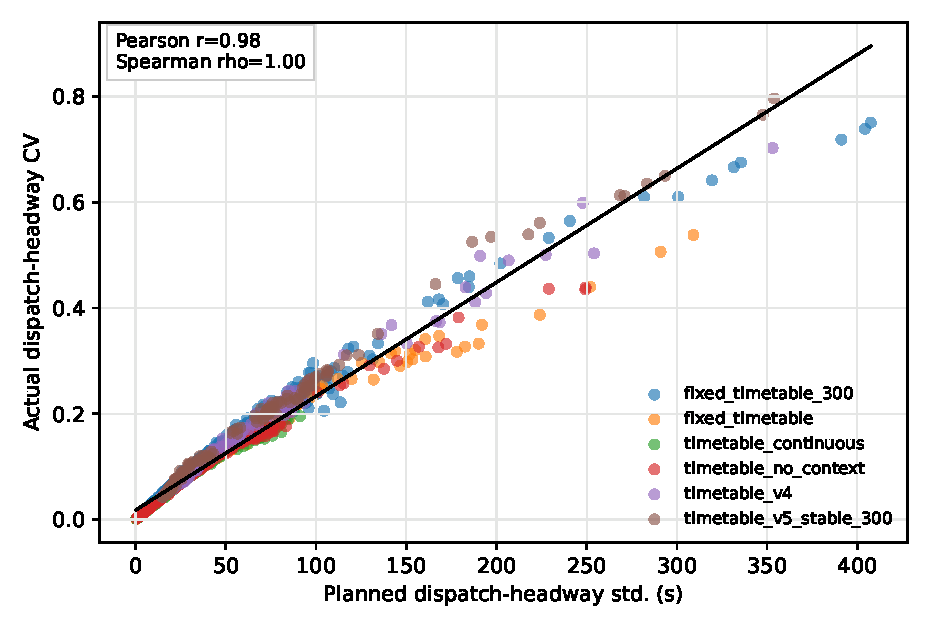
\includegraphics[width=0.62\textwidth]{figures/timetable_variance_correlation.pdf}
    \caption{Planned timetable variability versus realised dispatch-headway CV. Each point is one evaluation episode.}
    \label{fig:timetable_variance_correlation}
\end{figure}

\begin{table}[H]
\centering
\caption{Correlation between planned timetable variability and realised regularity (300 episode-level observations per method: 10 seeds $\times$ 30 final episodes).}
\label{tab:timetable_correlation}
\small
\begin{tabular}{@{}lcccc@{}}
\toprule
Method & Seeds & Observations & Pearson $r$ & Spearman $\rho$ \\
\midrule
Final rolling timetable & 10 & 300 & 0.994 & 0.981 \\
Wider-action rolling timetable & 10 & 300 & 0.990 & 0.998 \\
Continuous rolling timetable & 10 & 300 & 0.995 & 0.999 \\
No-context rolling timetable & 10 & 300 & 0.989 & 0.999 \\
Best fixed timetable SAC & 10 & 300 & 0.982 & 0.997 \\
Target-headway only & 10 & 300 & -- & -- \\
\bottomrule
\end{tabular}
\end{table}

The near-perfect correlations (Pearson $r > 0.98$ for all timetable variants) confirm that variation in the planned dispatch sequence is faithfully transmitted to realised dispatch regularity, validating the timetable channel as an effective control lever. The target-headway-only variant does not alter planned dispatch times and therefore cannot report this correlation.

\section{Discussion}
\label{sec:discussion}

\paragraph{Necessity of the timetable channel.}
The target-headway-only variant makes the upper decision useful to the lower controller by changing the lower target headway, but it does not alter planned dispatch times. That distinction matters: a target-headway setter can influence realised service through holding, but it does not itself optimise a timetable. In TransitDuet, the upper action defines a planned-headway adjustment that the simulator converts into a planned launch time. This makes the upper decision auditable through planned shifts, planned dispatch headways, and dispatch lateness, while the lower controller executes a dynamic timetable rather than inferring one indirectly.

\paragraph{Relation to conventional HRL.}
TransitDuet can be partially interpreted as a goal-conditioned lower controller because each active bus tracks the planned headway associated with its dispatched trip. A conventional option view does not, however, specify a rolling timetable generator. In TransitDuet, several planned headways remain active concurrently, and their effects overlap through shared fleet availability and station-level holding. The challenge is therefore not only that the two levels lack a common clock, but also that multiple timetable goals execute concurrently and credit must be assigned back to asynchronous dispatch-time decisions.

\paragraph{Interpreting joint training.}
The independent-assembly ablation is included because joint training is not automatically superior. If a fixed-timetable lower can be trained first and then paired with a timetable upper without loss, the appropriate contribution claim is a jointly trainable framework rather than that joint optimisation is always necessary. Conversely, if the jointly trained version improves total passenger time or dispatch feasibility, the result supports the stronger claim that the lower's adaptation to the rolling timetable is part of the gain.

\paragraph{Holding-delay trade-off.}
Bus holding methods can reduce out-of-vehicle wait and headway CV by increasing onboard delay. The evaluation therefore treats average holding time, onboard passenger time, and total passenger time as first-class metrics. A method that improves wait but worsens total passenger time should not be presented as an unqualified service improvement.

\paragraph{Baseline scope.}
The comparison includes timetable-search and bus-holding baselines. Daganzo-style and Xuan-style rules are standard analytical reference points for holding control. Holding-only SAC and same-simulator RL/MARL-style proxies compare TransitDuet with recent RL holding mechanisms without claiming exact reproduction of papers that use different networks, simulators, or demand models. This framing is deliberately conservative: same-simulator proxies test representative mechanisms, not whether TransitDuet supersedes every published implementation.

\paragraph{Limitations.}
The current experiments remain single-corridor simulations. Real transit networks introduce interlining, shared terminals, transfer passengers, driver relief constraints, and fleet rebalancing across routes. Scaling the timetable upper to such settings will require factored or graph-structured action representations. The simulator also abstracts away signal priority, incidents, driver heterogeneity, and endogenous passenger abandonment. Finally, the timetable experiments should be read as evidence from a ten-seed evaluation on one calibrated corridor; stronger external-validity claims require additional routes and paired tests on common held-out rollouts.

\section{Conclusion}
\label{sec:conclusion}

We have presented TransitDuet, a bi-level reinforcement learning framework for dynamic bus timetable optimisation and real-time holding control.
The dynamic timetable channel (Section~\ref{sec:tap}) links dispatch planning and station holding: the upper policy selects planned-headway adjustments, and the lower policy regulates holding actions against the resulting trip-specific targets.
Fleet-size feasibility is maintained through online gradient descent penalty adaptation at the upper level, while Lagrangian relaxation preserves headway regularity at the lower level.

On a calibrated 22-station corridor with stochastic demand and elastic fleet budgets, TransitDuet achieves a mean composite cost 3.2\% below the target-headway-only variant and 11.5\% below the best fixed-timetable baseline, with a mean total passenger time of 18.15 minutes across ten random seeds.
Timetable ablations confirm that the discrete action grid, lower-state context, and joint training each contribute to these gains.

Future work should test TransitDuet on multi-route networks with shared fleets and transfer coordination. Deployment through a calibrated digital twin with domain randomisation could assess robustness to traffic signals and driver heterogeneity. Real-time demand forecasting and passenger-demand elasticity would further connect service quality to ridership.


\appendix
\section{Hyperparameter details}
\label{app:hyperparams}

\Cref{tab:hyperparams_full} lists the hyperparameters of the final rolling-timetable configuration used for the main TransitDuet results.

\begin{table}[H]
\centering
\caption{Complete hyperparameter specification.}
\label{tab:hyperparams_full}
\footnotesize
\setlength{\tabcolsep}{2pt}
\begin{tabular}{@{}p{0.14\textwidth}p{0.24\textwidth}p{0.17\textwidth}p{0.38\textwidth}@{}}
\toprule
Group & Parameter & Value & Description \\
\midrule
\multirow{4}{*}{Environment}
  & Route speed noise        & 1.5    & Log-normal speed noise $\sigma$ \\
  & Maximum active buses     & 25     & Hard cap on concurrent buses ($> \Nfleet^{\max}$) \\
  & Trips per service day & 264   & Total trips per service day \\
  & Demand multiplier standard deviation & 0.15 & Per-hour demand multiplier standard deviation \\
\midrule
\multirow{15}{*}{Upper policy}
  & State dimension    & 11             & System summary (5), HoldFB (3), and trip context (3); see Eq.~\ref{eq:upper_state} \\
  & Action bins  & 5 bins         & $\Delta h \in \{-60,-30,0,30,60\}$\,s \\
  & Minimum shift   & $-60$          & Seconds \\
  & Maximum shift  & $+60$          & Seconds \\
  & Hidden-layer width   & 64             & MLP hidden-layer width \\
  & Learning rate            & $3 \times 10^{-4}$ & Policy and critic learning rate (Adam) \\
  & Mini-batch size   & 64             & Replay-buffer mini-batch \\
  & Updates per episode & 10     & SAC gradient steps per training episode \\
  & Replay capacity      & 50{,}000 & Upper transitions stored \\
  & Critic ensemble size $K$    & 10     & RE-SAC critic ensemble size \\
  & $\beta_{\mathrm{LCB}}$         & $-2.0$ & LCB coefficient in policy improvement \\
  & $\gamma_{\mathrm U}$           & 0.95   & Discount factor (per-dispatch) \\
  & $\alpha_{\max}^{\mathrm U}$    & 0.06   & Maximum entropy temperature (auto-tuned) \\
  & $\Nfleet^{\min},\Nfleet^{\max}$ & $8, 16$ & Elastic fleet sampling range \\
  & $\Nfleet$ (default)    & 12             & Soft fleet target (overshoot$^2$ penalty) \\
\midrule
\multirow{14}{*}{Lower policy}
  & Hidden-layer width     & 64      & MLP hidden-layer width \\
  & Action bins    & 8 bins  & Holding action $\in \{0,3,6,9,12,15,20,30\}$\,s \\
  & $\climit$                & 0.5     & Lagrangian cost budget \\
  & Mini-batch size     & 512     & Replay-buffer mini-batch \\
  & Updates per episode & 30 & SAC gradient steps per training episode \\
  & Learning rate              & $3 \times 10^{-4}$ & Critic and policy learning rate \\
  & $\lambda_{\text{lr}}$    & $10^{-4}$ & Lagrangian multiplier learning rate \\
  & $\gamma$                 & 0.99    & Discount factor \\
  & $\tau$                   & 0.005   & Soft target update rate \\
  & Automatic entropy tuning   & true    & Automatic entropy tuning \\
  & $\alpha_{\max}^{\mathrm L}$ & 0.08  & Maximum entropy temperature \\
  & Critic ensemble size $K$ & 10   & RE-SAC critic ensemble size \\
  & $\beta_{\mathrm{ood}}$   & 0.1     & Ensemble-spread regulariser weight \\
  & Reward scale   & 1.0     & Reward scaling factor \\
\midrule
\multirow{7}{*}{Coupling}
  & $e_{\mathrm{warm}}$       & 15 episodes   & Lower-only warmup ($\Delta h = 0$) \\
  & $\alpha_{\mathrm H}$      & 0.5           & Hindsight-credit weight (Eq.~\ref{eq:hindsight_reward}) \\
  & TPC $\epsilon$            & 0.25          & Behavior-mixture exploratory probability \\
  & TPC $\sigma_{\mathrm{tgt}}$ & 20 s        & Target-mode Gaussian standard deviation \\
  & TPC $w_{\max}$            & 5             & Importance-sampling weight clip \\
  & TPC moving-average rate $\tau$ & 0.005     & Polyak rate of exponential-moving-average target upper \\
  & $\eta_{\thetavec}$        & 0.01          & ApproPO $\thetavec$-OGD step size \\
\midrule
\multirow{3}{*}{Training}
  & Training episodes       & 300     & Total training episodes per seed \\
  & Checkpoint interval            & 50      & Episodes \\
  & Lower replay capacity  & $5 \times 10^{5}$ & Lower replay-buffer capacity \\
\bottomrule
\end{tabular}
\end{table}

%% ---------------------------------------------------------------
\section{Environment details}
\label{app:env}

The simulation models a single bidirectional bus route calibrated from operational data of an urban bus corridor.

\paragraph{Route topology.}
The route comprises $M$ stations connected by inter-station segments.
Each direction (upstream and downstream) traverses all $M$ stations in sequence, with terminal turnaround at each end.
Station positions and inter-station distances are read from operational records, and segment-level speed profiles are specified per hour of day.

\paragraph{Stochastic travel speed.}
Inter-station travel times are driven by a stochastic speed model.
At each route-state update, the speed limit on segment $(i, i{+}1)$ is drawn as
\begin{equation}
  v_{i} = \min\!\bigl(V_{\max},\;\max\bigl(0,\;\lfloor\ln\mathcal{LN}(\mu_i(t),\,\sigma)\rfloor\bigr)\bigr),
\end{equation}
where $\mu_i(t)$ is the historical mean log-speed for segment~$i$ at hour~$t$, $\sigma = 1.5$ is the log-normal dispersion parameter, and $V_{\max}$ is the segment maximum speed.
This produces realistic speed variability that induces headway deviations even under a well-designed timetable.

\paragraph{Passenger generation.}
Passenger arrivals follow a Poisson process governed by time-varying origin--destination (OD) matrices.
The OD data specifies hourly demand rates between all station pairs.
At each simulation second, for every origin station with non-zero demand to a given destination, a Poisson draw with rate $\lambda_{od}/3600$ determines the number of new passengers.
Each passenger records an appearance time, an origin, and a destination; waiting time is measured from appearance to boarding.

\paragraph{Bus operations.}
Each bus maintains a state machine with four phases:
\begin{enumerate}
  \item Holding: the bus is held at a station for the duration specified by the lower-level policy (0--30\,s in the final configuration).
  \item Dwelling: passengers alight and board. Boarding proceeds until the bus reaches capacity ($C = 50$ passengers) or no more waiting passengers have a valid destination downstream.
  \item Travel: the bus moves toward the next station at the current stochastic speed. Acceleration ($3\;\text{m/s}^2$) and deceleration ($5\;\text{m/s}^2$) are modeled at departure and arrival.
  \item Waiting for action: upon arriving at a station, the bus waits for the next holding action from the lower-level policy.
\end{enumerate}
Forward and backward headways are computed with respect to the preceding and following buses in the same direction, and the headway deviation from the target set by the upper policy defines the per-step cost (\Cref{eq:lower_cost}).

\paragraph{Timetable structure.}
A service day consists of 264 trips alternating between the two directions, truncated from a full operational schedule to keep simulation tractable.
At most 25 buses may be concurrently active.
In the main configuration, the upper policy selects a planned-headway adjustment for the next same-direction trip. The simulator converts the resulting planned headway into a planned launch time and dispatches the trip once the planned time and vehicle-availability constraints are satisfied. The baseline timetable is retained only as a reference for reporting planned shifts and deviations.

\paragraph{Episode termination.}
An episode ends when all 264 trips have been launched and every bus has completed its trip (i.e., no bus remains on-route). At this point the measurement vector $\zvec$ (\Cref{eq:measurement}) is computed for the ApproPO $\thetavec$-OGD update.

%% ---------------------------------------------------------------
\section{Network architectures}
\label{app:networks}

All networks use rectified linear unit (ReLU) activations and are trained with Adam. Weight initialization follows PyTorch defaults unless otherwise noted.

\paragraph{Upper policy $\piU$ (categorical timetable action).}
A two-layer multilayer perceptron (MLP) maps the 11-dimensional upper state (5 system summary dimensions + 3 holding-feedback dimensions + 3 trip-context dimensions; \cref{eq:upper_state}) to logits over five planned-headway adjustments $\Delta h \in \{-60,-30,0,30,60\}$\,s:
\begin{center}
\small
\begin{tabular}{lll}
\toprule
Layer & Shape & Activation \\
\midrule
Linear & $11 \to 64$ & ReLU \\
Linear & $64 \to 64$ & ReLU \\
Logit head & $64 \to 5$ & Softmax for sampling \\
\bottomrule
\end{tabular}
\end{center}
The selected bin defines $h^{\mathrm{plan}}=\mathrm{clip}(300+\Delta h,240,360)$\,s. The simulator then sets the next same-direction planned launch time to the maximum of the previous actual dispatch plus $h^{\mathrm{plan}}$ and the current time plus a 60\,s notice window. The continuous upper policy remains available as the continuous rolling-timetable ablation.

\paragraph{Lower policy $\piL$ (categorical holding action).}
A two-layer MLP maps the lower state to logits over eight holding bins $\{0,3,6,9,12,15,20,30\}$\,s:
\begin{center}
\small
\begin{tabular}{lll}
\toprule
Layer & Shape & Activation \\
\midrule
Linear & $(13{+}K) \to 64$ & ReLU \\
Linear & $64 \to 64$ & ReLU \\
Logit head & $64 \to 8$ & Softmax for sampling \\
\bottomrule
\end{tabular}
\end{center}
The additional five lower-state dimensions are the previous holding action, the current trip's planned headway, the previous and next planned same-direction gaps, and the station phase. The same network is shared across all buses, with bus-specific behavior arising from heterogeneous input states.

\paragraph{Reward Q-ensemble $\{Q_k\}_{k=1}^{K}$ (RE-SAC, $K{=}10$).}
The lower replaces the standard twin-Q SAC critic with an ensemble of $K{=}10$ independently initialized Q-networks. The policy is improved against a lower-confidence-bound (LCB) value $\bar{Q} + \beta_{\mathrm{LCB}} \sigma_Q$ with $\beta_{\mathrm{LCB}} = -2$, computed across the ensemble at every gradient step. Each ensemble member shares the same MLP shape:
\begin{center}
\small
\begin{tabular}{lll}
\toprule
Layer & Shape & Activation \\
\midrule
Linear & $(13{+}K{+}1) \to 64$ & ReLU \\
Linear & $64 \to 64$ & ReLU \\
Linear & $64 \to 1$ & --- \\
\bottomrule
\end{tabular}
\end{center}
Each $Q_k$ takes the concatenation of the lower state and scalar action as input. All members share a common mean target $(1/K)\sum_k \bar{Q}_k$ during temporal-difference learning to prevent ensemble divergence. The per-Q mean-squared-error (MSE) loss is augmented with a small ensemble-spread penalty $\beta_{\mathrm{ood}}\,\mathrm{std}_k(Q_k)$ ($\beta_{\mathrm{ood}}{=}0.1$) that encourages disagreement on out-of-distribution actions. All ensemble members have exponential-moving-average target networks with Polyak rate $\tau = 0.005$. We use a Q-ensemble rather than a twin Q to construct lower-confidence bounds; the twin-Q variant in standard SAC corresponds to $K{=}2$ without the LCB.

\paragraph{Cost Q-network $Q_c$.}
A single MLP with the same MLP shape as one ensemble member estimates the expected cumulative cost (headway deviation) under the current policy:
\begin{center}
\small
\begin{tabular}{lll}
\toprule
Layer & Shape & Activation \\
\midrule
Linear & $(13{+}K{+}1) \to 64$ & ReLU \\
Linear & $64 \to 64$ & ReLU \\
Linear & $64 \to 1$ & --- \\
\bottomrule
\end{tabular}
\end{center}
The cost critic is trained with the same target-network mechanism and soft update rate as the reward critics.
Its output enters the policy loss through the Lagrangian multiplier $\lambda$: the policy minimises $\alpha \log \pi - Q + \lambda Q_c$.

%% ---------------------------------------------------------------
\section{Auxiliary hindsight credit: derivation and contrast with cross-advantage}
\label{app:coupling_derivation}

The main cross-level coupling in TransitDuet is the rolling timetable channel of \cref{sec:tap}. This appendix derives the auxiliary hindsight credit on the upper reward (Eq.~\ref{eq:hindsight_reward} in \cref{sec:tap}), an upper-only signal for per-dispatch credit assignment. It also contrasts this mechanism with a literal asynchronous extension of the cross-advantage objective of Pan et al.~\citep{pan2024roboduet}.

\subsection{Synchronous cross-advantage (RoboDuet, background)}

In the synchronous setting of Pan et al.~\citep{pan2024roboduet}, two agents act at every time step $t$ on a shared state $s_t$. The cross-advantage augmented objective is
\begin{equation}
  \mathcal{L}_{\text{upper}}^{\text{sync}} = -\mathbb{E}_{t}\bigl[(A_{\mathrm{U}}(s_t, a_t^{\mathrm{U}}) + \beta\, A_{\mathrm{L}}(s_t, a_t^{\mathrm{L}}))\,\nabla\!\log\piU(a_t^{\mathrm{U}} \mid s_t)\bigr],
  \label{eq:roboduet_upper}
\end{equation}
which is well-defined because both advantages are evaluated at the same shared state-action pair.

\subsection{The asynchrony challenge}

In TransitDuet, $\piU$ acts at dispatch events $\{t_1^{\mathrm{U}}, \ldots, t_N^{\mathrm{U}}\}$ while $\piL$ acts at station arrivals $\{t_1^{\mathrm{L}}, \ldots, t_M^{\mathrm{L}}\}$ with $M \gg N$, on disjoint event sets and different state spaces. There is no single time step at which $\AU$ and $\AL$ are jointly defined on a shared state, so the direct sum in Eq.~\eqref{eq:roboduet_upper} is undefined.

\subsection{Trip-lifecycle alignment and the realised gap}

We resolve this through trip-lifecycle alignment. Each upper action $a_{\mathrm{U},i}$ after dispatch $i-1$ selects the planned-headway adjustment that determines the planned launch time and planned headway for trip $i$. The realised inter-dispatch gap is the elapsed time between consecutive bus departures after vehicle availability and holding interactions are applied:
\begin{equation}
  g_i = t_{\mathrm{actual},i+1} - t_{\mathrm{actual},i},
\end{equation}
computed per direction so that buses operating on opposite legs do not interleave. The per-direction mean and standard deviation of $\{g_i\}$ define the deviation
\begin{equation}
  \Delta_i = \frac{|g_i - \bar{g}|}{\sigma_g}.
  \label{eq:gap_dev}
\end{equation}

\subsection{Hindsight-credited upper reward}

The upper reward at dispatch $i$ is the sum of the episode-level system reward (a belief-weighted MORL scalarisation of wait, fleet overshoot, and headway CV; Eq.~\ref{eq:morl_reward}) and a per-dispatch hindsight credit derived from $\Delta_i$:
\begin{equation}
  R_{\mathrm{U}}^{(i)} = R_{\mathrm{sys}}(\zvec) - \alpha_{\mathrm{H}} \cdot \frac{\Delta_i - \bar{\Delta}}{\sigma_{\Delta}}, \qquad \alpha_{\mathrm{H}} = 0.5.
  \label{eq:hindsight_reward_app}
\end{equation}
The credit is recentered per episode so that dispatches with above-average gap deviation receive a negative credit and dispatches with below-average deviation receive a positive one. The system reward is shared across all dispatches in an episode.

\subsection{Why we did not use literal cross-advantage}

A literal asynchronous extension of Eq.~\eqref{eq:roboduet_upper} would aggregate per-trip lower advantages into the upper objective:
\begin{equation}
  \tilde{R}^{\text{lit},(i)}_{\mathrm{U}} = R_{\mathrm{U}}^{(i)} + \beta \cdot \tfrac{1}{|\mathcal{J}(i)|}\sum_{j \in \mathcal{J}(i)} A_{\mathrm{L}}(s_{\mathrm{L},j}, a_{\mathrm{L},j}),
  \label{eq:cross_adv_literal}
\end{equation}
where $\mathcal{J}(i)$ is the set of lower-level transitions during trip~$i$. An early prototype of this objective was unstable in our runs. The per-step lower advantage and the per-dispatch upper advantage differed in scale by 1--2 orders of magnitude across a trip lifecycle. A single scalar $\beta$ therefore either suppressed the cross-level signal or destabilised lower training. In addition, the lower advantage estimator uses an LCB-discounted ensemble Q (\cref{sec:lower}), which is a nonlinear function of the policy parameters. The simple unbiasedness argument for the synchronous setting therefore does not transfer directly. The hindsight-credit formulation in Eq.~\eqref{eq:hindsight_reward_app} instead injects the per-trip execution outcome (gap regularity) into upper credit assignment without requiring lower-advantage backflow.

\subsection{What changes for our off-policy SAC upper}
The TransitDuet upper is trained as RE-SAC (\cref{sec:upper}, Eqs.~\ref{eq:upper_q_target}--\ref{eq:upper_policy_loss}), not as REINFORCE. Each per-dispatch transition is pushed to a replay buffer, and the policy and critic are updated by repeated mini-batch SAC gradient steps. The REINFORCE-based unbiasedness argument for a synchronous on-policy estimator is therefore not the appropriate analytical lens for this setup. The lower is also updated between upper SAC gradient steps, so the upper training distribution is non-stationary. The timetable ablations evaluate whether joint training is necessary or whether a frozen independently trained lower is sufficient. The upper ensemble-LCB Q value penalises epistemic uncertainty in its off-policy training objective.

% Keep all figures and tables out of the reference list.
\clearpage
\FloatBarrier

\bibliographystyle{vancouver}
\bibliography{references}

\end{document}
